\chapter{GAMESS}

\section{Introduction}

GAMESS (General Atomic and Molecular Electronic Structure System) is an ab initio quantum chemistry software that allows a wide variety of calculations, including Hartree-Fock (HF), density functional theory (DFT), Møller–Plesset perturbation theory (MP2), configuration interaction (CI), and more.

\section{Installation on Linux}

Follow the official installation guide:

\begin{itemize}
  \item Download the source code from \url{https://www.msg.chem.iastate.edu/GAMESS/}
  \item Unpack and run the \texttt{config} script to set system variables.
  \item Use \texttt{cmake} or \texttt{make} with appropriate options for linking LAPACK, BLAS, and MPI.
  \item Use OpenBLAS or MKL for optimized linear algebra routines.
\end{itemize}

Example:

\begin{verbatim}
export GMS_PATH=$HOME/gamess
cd $GMS_PATH
./config
make ddi
make modules
make gamess
\end{verbatim}

\section{Running on Clusters}

You need to load the correct environment modules:

\begin{verbatim}
module load gcc
module load openmpi
module load openblas
\end{verbatim}

Run using:

\begin{verbatim}
rungms molecule.inp > molecule.log
\end{verbatim}

Or submit with SLURM/PBS scripts:

\begin{verbatim}
#!/bin/bash
#PBS -N gamess_job
#PBS -l nodes=1:ppn=8
cd $PBS_O_WORKDIR
rungms input.inp > input.log
\end{verbatim}

\section{Running on Windows (WSL)}

Install WSL and compile GAMESS in Ubuntu. Use the same Linux procedure. Use MobaXterm or VSCode for integration and job control.

\section{Analysis and Output Files}

Output files:

\begin{itemize}
  \item \texttt{.log} – standard output
  \item \texttt{.dat} – data files (e.g., orbital info)
  \item \texttt{.trj} – trajectory (if MD is used)
\end{itemize}

\section{Useful Links}

\begin{itemize}
  \item Official site: \url{https://www.msg.chem.iastate.edu/GAMESS/}
  \item Manual: \url{http://www.msg.chem.iastate.edu/gamess/GAMESS_Manual.pdf}
\end{itemize}


\section{Nonadiabatic Dynamics with GAMESS}

\subsection*{Overview}

Nonadiabatic dynamics (NAMD) with GAMESS can be performed using MRSF-TDDFT gradients and Newton-X as a driver. The goal is to simulate electronic transitions (e.g., S2 → S1 → S0) along nuclear trajectories with surface hopping.

\subsection*{Initial Condition Generation}

Initial conditions are prepared using Wigner sampling, usually via Newton-X. You may also use GAMESS jobs followed by extraction scripts to set geometries and momenta.

\subsection*{Running the Dynamics}

Use a Python script or shell wrapper to loop over multiple trajectories:

\begin{verbatim}
for i in {1..50}; do
  cd traj_$i
  ./run_namd.sh
done
\end{verbatim}

Each trajectory should call GAMESS with MRSF-TDDFT gradients and pass output to Newton-X or internal scripts.

\subsection*{Restarting Simulations}

Check for failures and re-submit with:

\begin{verbatim}
grep "NAMD step" traj_*/log | awk '{print $1}' > failed.txt
# then resubmit failed cases
\end{verbatim}

\subsection*{Population and Bond Analysis}

You may analyze population evolution of S0–S3 states using CSV outputs. Plot with gnuplot or matplotlib.

\begin{figure}[h]
    \centering
    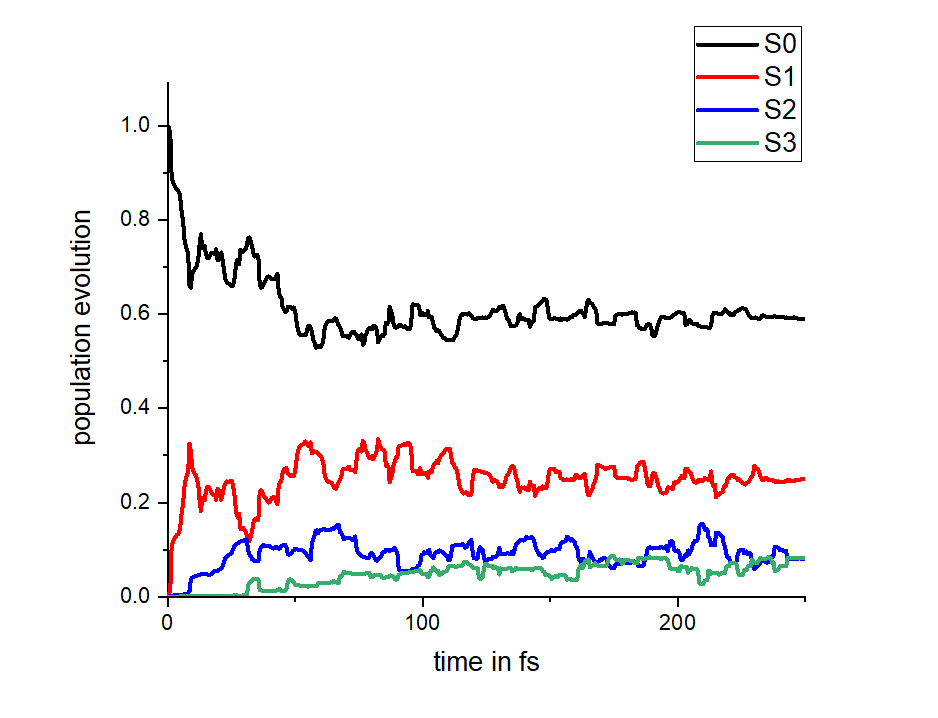
\includegraphics[width=0.8\textwidth]{docs/img/population_evolution.png}
    \caption{Electronic state population during NAMD}
\end{figure}

Similarly, compute dissociation fraction based on bond distance criteria:

\begin{figure}[h]
    \centering
    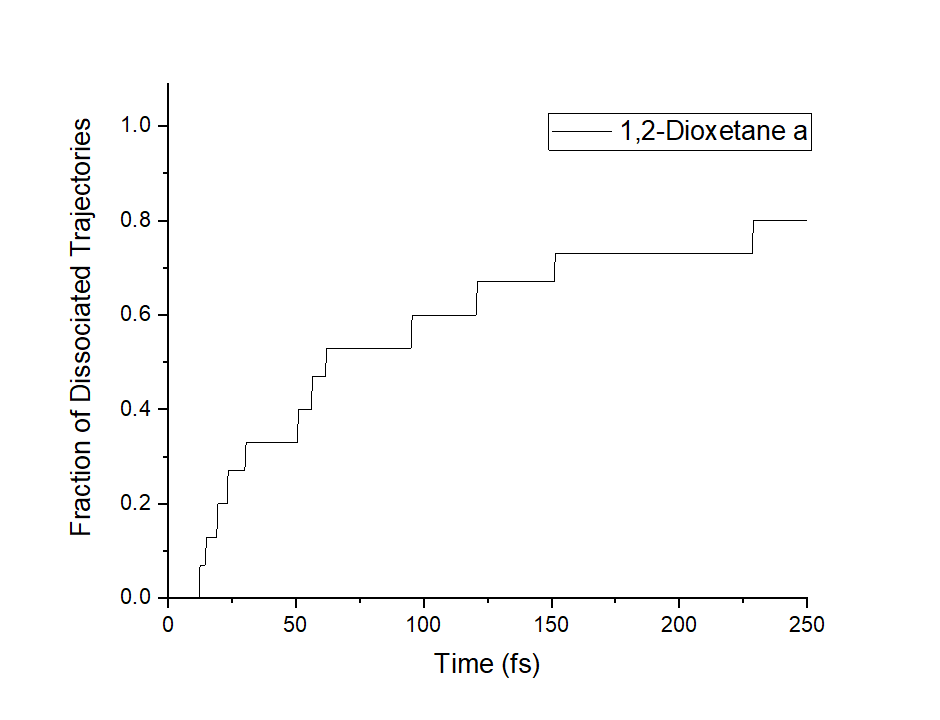
\includegraphics[width=0.8\textwidth]{docs/img/dissociation_fraction.png}
    \caption{Fraction of dissociated molecules over time}
\end{figure}

Bond lengths like C1–C2 can be tracked for geometric analysis:

\begin{figure}[h]
    \centering
    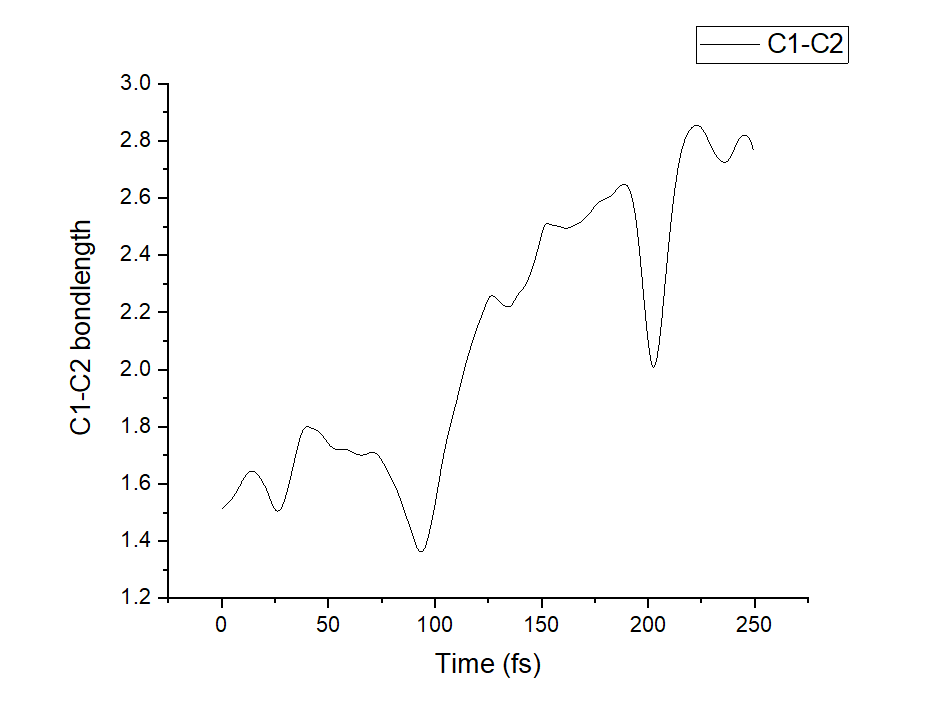
\includegraphics[width=0.8\textwidth]{docs/img/c1_c2_distance.png}
    \caption{Distance between C1 and C2 atoms vs. time}
\end{figure}

\subsection*{Output Evaluation}

Use Python scripts to extract:
\begin{itemize}
  \item Orbital occupations
  \item Excitation character
  \item CI vector contributions
\end{itemize}

Tools:
\begin{itemize}
  \item \texttt{mci-flu-script-stable.py}
  \item \texttt{ESoccupationextract-stable.py}
  \item Jupyter Notebooks for population plotting
\end{itemize}
